\chapter{遗传密码}
\label{chap:chapter8}
\minitoc

到现在为止,我们已经使用Perl进行了基序的查找、模拟DNA突变、生成随机序列,以及把DNA转录成RNA。这些都是非常重要的主题,它们可以作为你在研究生物学系统过程中使用到的计算技术的好的入门指引。

在本章中,我们将编写Perl程序,来模拟遗传密码是如何指导DNA翻译成蛋白质的。开始我先介绍散列这种数据类型。之后,在对不同的数据结构(散列、数组和数据库)如何对实验信息存取进行简要的讨论后,我们将编写一个程序,来把DNA翻译成蛋白质。我们也将继续探讨正则表达式,并编写处理FASTA文件的代码。

\section{散列}
在Perl中有三种主要的数据类型。你已经学习了其中的两种:标量变量和数组。现在,我们将开始学习第三种:\textit{散列}(也叫做关联数组)。

散列提供了与键相关联的值的快速查找。举个例子,比如说你有一个叫做 \verb|%english_dictionary|的散列。(是的,散列以百分号起始。)如果你想查找单词“recreant”的定义,可以这样:

\begin{lstlisting}
$definition = $english_dictionary{'recreant'};
\end{lstlisting}

标量 \verb|'recreant'|是键,返回的标量定义是值。就像你在这个例子中看到的这样,当你访问单个元素时,散列(就像数组那样)把起始的字符换成了美元符号,因为散列查找返回的值是一个标量值。通过它们使用的括号类型,你可以把散列查找和数组元素区分开来:数组使用中括号[ ],而散列使用大括号{ }。

如果你想给键赋值,只需要一个类似的简单语句:

\begin{lstlisting}
$english_dictionary{'recreant'} = "One who calls out in surrender.";
\end{lstlisting}

此外,如果你想用一些键值对初始化一个散列,方法类似于初始化数组,不同的是每一对都成了键-值对:

\begin{lstlisting}
%classification = (
  'dog',      'mammal',
  'robin',    'bird',
  'asp',      'reptile',
);
\end{lstlisting}

它用值 \verb|'mammal'|对键 \verb|'dog'|进行了初始化,依此类推。还有另一种书写方法,可以使其含义更加清晰一些。下面这些代码所做的事情和前面的代码完全一样,但把键-值的关系表现地更加明确一些:

\begin{lstlisting}
%classification = (
  'dog'   => 'mammal',
  'robin' => 'bird',
  'asp'   => 'reptile',
);
\end{lstlisting}

你可以得到散列的所有键构成的数组:

\begin{lstlisting}
@keys  = keys %my_hash;
\end{lstlisting}

你也可以得到散列的所有值构成的数组:

\begin{lstlisting}
@values  = values %my_hash;
\end{lstlisting}

在许多不同的情形下你都会用到散列,尤其是当你的数据以键-值形式存在时,或者你需要快速查找到某个键的值时。举个例子,在本章的后面部分,我们将编写程序,使用散列来提取一个基因的信息。基因的名字就是键,关于基因的信息就是键的值。从数学上来讲,一个Perl散列表示的永远是一个有穷函数。

“散列”这个名字来源于散列函数,如果你留心去寻找,几乎关于算法的任何一本书中都会对它进行定义。让我们跳过它们深层次的工作细节,只讨论它们的表现。

\section{生物学的数据结构和算法}
生物学家研究生物学数据,并且试图阐明在生命系统中基于它的存在结构是如何发挥功能的。生物信息学常被用来尽可能地对这样的存在结构进行建模。(不要太咬文嚼字了,我只是概括而言的!)

生物信息学也会采取略有不同的方案。它会考虑对于这些数据可以做什么,然后尝试去阐明如何对它们进行组织才能实现目标。换句话说,通过以一种方便的数据结构来表征数据,它会尝试去产生一种算法。

既然你已经学习了Perl中的三种数据类型,就是标量、数组和散列,现在是时候来看一下与算法和数据结构相关的主题了。在\autoref{chap:chapter3}中,我们已经讨论了算法。现在讨论的重点就是算法中数据组织形式的重要性,换言之,就是算法中的数据结构。

此处最为关键的一点是,不同的算法通常需要不同的数据结构。

\subsection{基因表达数据库}
让我们考虑一个典型问题。假设你在研究一种生物,它总共大约有30,000个基因。(是的,没错,这就是人类。)假设你正在研究一种类型的细胞,在某个特定的环境条件下它还没有被深入研究过,你想知道,对于每一个基因来说,它是否表达了。\footnote{对于非生物学家:当一个基因转录成RNA后,就可以进一步翻译出蛋白质了,就说这个基因表达了。}你有一个很好的芯片设备,它把那个细胞的表达信息都告诉你了。现在,对于每一个基因,你要去查找一下看看在细胞中它是否表达了。你必须在你的网站上实现这种查找功能,这样在你即将发表的文章中看到你结果的访问者就可以找到基因的表达数据了。

有许多不同的方法可以实现。让我们看一下几个不同的实现方法,作为对算法和数据结构的艺术和科学的简洁的入门介绍。

你的数据是什么?为简单起见,假设你有这个生物所有基因的名字,以及在你的实验中表示表达水平的基因的表达数值。所有未表达的基因的表达数值都是0。

\subsection{使用未排序数组的基因表达数据}
现在,假设你想知道基因是否表达了,而不是具体的表达水平,并且你想使用数组来解决这个编程问题。毕竟,现在你已经对数组非常熟悉了。你该怎么做呢?

你可能只在数组中存储那些表达基因的基因名,而丢弃其他的基因名。假如有8,000个表达基因。之后,要进行任何查询,只需要遍历数组,把查询的基因名和数组中的每一个基因名进行比较,直到你找到它或者没有找到它但已经到达了数组的末尾。

这样是可行的,但也存在问题。最主要的,它非常慢。如果你只是偶尔查询一下,这并不是问题,但如果有许多人访问你的网站对这套新的表达数据进行查询,问题就大了。平均来说,查找一个表达基因需要遍历4,000个基因名字,而查找一个未表达的基因则需要进行8,000次比较。

此外,如果某个人查找的是你的研究中没有的一个基因,因为你丢弃了所有未表达基因的基因名,所以你就没法对其进行回应。查询给出的结果是没有找到这个基因,而不是说要查询的基因并不在你的实验结果中的错误信息。如果要查询的基因虽然并不在你的研究结果中,但却在这类细胞中表达(你刚好错过了它),那这个查询就是一个假阴性了。你可能更希望遇到这种情况时,你的程序可以报告给用户,说那个名字的基因并没有在实验中被研究。

所以你打算把30,000个基因都存储到数组中。(当然,现在进行查找会更慢一些。)但是,如何把表达基因和未表达基因区分开来呢?你可以把每个基因的名字都存储到数组中,并且把表达测量值附加到每个基因名的后面,然后你就可以准确无误的知道某个基因是不是在你的实验中并不存在了。

然而,这个程序仍然有点慢。你仍然不得不去遍历整个数组,直到你找到那个基因或者确定它并没有被研究为止。如果它是数组中的第一个元素,你立马就可找到它,否则你可能不得不等到它遍历到数组的最后一个元素。平均来说,你将不得不遍历一半的数组。另外,你还不得不把需要查找的基因名和数组中的基因名一个一个进行比较。对于每次查询来说,平均都要进行15,000次的比较,这非常慢。(实际上,在现代的计算机上,这其实也并不是慢的可怕。但是我想指出这一点,这样的东西确实意味着一个运行很慢的程序。)

另外一个问题就是,在一个标量中你存储了两个值:基因名和表达测量值。处理这样的数据,你必须还要把基因名和基因的表达测量值分割开来。

虽然有这些缺点,但这种方法确实是可行的。现在,我们来讨论一下另外一种方法。

\subsection{使用排序数组和折半查找的基因表达数据}
你可能尝试把所有的基因名按照字母顺序排序后存储在数组中,然后使用下面这种查找技术。首先,看一下中间的元素。(就像我们已经看到的,使用 \verb|scalar @array|表达式你可以得到数组的大小)。按照字母顺序,如果你的基因名排在中间元素的前面,你就可以忽略数组的后半部分了,并找到数组剩余的前半部分的中间元素。如此循环往复,每一步都可以把查找范围缩小到前一步元素数目的一半,直到最终找到对应的匹配,或者发现根本不存在。下面是用伪代码进行实现:

\begin{lstlisting}
Given a sorted array, and an element:

Until you find the element or discover it's not there,

  Pick the midpoint of the array, $array[scalar(@array)/2]

  Compare your element with the element at the midpoint

  If that matches your element, you're done.

  Else, ignore the half of the array that your element is not in
}
\end{lstlisting}

在Perl中要按照字母顺序比较两个字符串,你可以使用\textit{cmp}操作符,如果两个字符串一样它会返回0,如果它们按照字母顺序排列就会返回-1,如果它们按照字母顺序的逆序排列就会返回1。比如,下面这个会返回0:

\begin{lstlisting}
'ZZZ' cmp 'ZZZ';
\end{lstlisting}

这个返回-1:

\begin{lstlisting}
'AAA' cmp 'ZZZ';
\end{lstlisting}

最后,这个返回1:

\begin{lstlisting}
'ZZZ' cmp 'AAA';
\end{lstlisting}

这种算法叫做\textit{折半查找},它会明显提高在数组中进行查找的速度。比如,要查找30,000个基因,最多只需要大约15次的循环即可。(和未排序数组平均进行15,000次的比较相比。)当然,你还必须要对列表进行排序,这也需要一定的时间。如果你需要不停地增加元素,你就不得不把它们插入倒合适的位置,或者把它们添加到末尾然后对整个数组进行重新排序。所有这样的插入或者排序都可能会相当的慢。但是,如果你仅需要进行一次排序,然后进行大量的查找,折半查找还是值得考虑的。

既然我们已经谈到了它,就来看看如何对数据进行排序。这是按照字母顺序对由字符串构成的数组进行排序的方法:

\begin{lstlisting}
@array = sort @array;
\end{lstlisting}

这是以升序对由数字构成的数组进行排序的方法:

\begin{lstlisting}
@array = sort { $a <=> $b } @array;
\end{lstlisting}

还可以进行多种其他形式的排序,但这些是最常见的。更多的细节,可以参看Perl文档中关于\textit{sort}函数的说明。

\subsection{使用散列的基因表达数据}
你还可以使用散列来查找你数据中的某个基因。要实现这一点,你需要以基因名作为键、以表达测量值作为值载入散列。然后对散列一个简单的调用,使用待查找基因的基因名作为键,就可以返回这个基因的实验结果,这就是你要的答案。与把基因名和表达值存储到一个标量字符串中相比,这个过程要清晰多了。在这里,键是一个标量,而值则是另外一个标量。

此外,取决于散列的构建方式,你可以很快得到你要的答案,因为现在的散列都不需要进行繁琐的查找就可以找到某个键的值。使用散列通常要比折半查找快很多。此外,你还可以知道查找的基因在数据中是否存在,因为你可以明确询问某个散列值是否被定义了,就像这样:

\begin{lstlisting}
if( defined $myhash{'mykey'}  ) { ... }
\end{lstlisting}

另外,如果你开启了警告模式,你会得到一个错误信息,因为你提到的是一个未定义的值。

相比于折半查找,散列的另一个优势在于,你可以向散列中添加或删减元素,而不需要对整个数组进行重排序。

最后,因为散列是作为一个基本的数据类型内置在Perl中的,所以它们非常容易使用,而且你不需要进行太多的编程就可以实现你的目的。通常情况下,节省编程的时间要比节省程序运行的时间更加重要一些。我在\autoref{chap:chapter3}中提到过这一点,但此处还是有必要强调一下。对于一个程序员来说,懒惰的方法通常都是最有效的方法:让机器来干活吧!

但是,不要想当然的认为散列永远都是最好的方法。比如,散列并不以排序的顺序存储其中的元素,所以如果你需要以排序的方式查看数据,就不得不对它进行明确的排序,就像这样:

\begin{lstlisting}
@sorted_keys = sort keys %my_hash;
\end{lstlisting}

这样就可以了,但对于大的数组来说,它可能会有点慢。(当然,你也可以对值进行排序。)

对于这个表达数据的例子,我们总结一下关于数据结构的讨论,下面是对Perl中不同数据结构属性的信息描述,包括对基因名数据集进行的查找、添加和删减、以及保持排序顺序:

\begin{itemize}
  \item 如果你只需要看看某个东西是不是在数据集中,并不需要按照顺序把它们罗列出来,那就使用散列。
  \item 如果你需要一个排序的数据集以及相对快速的查找,而不需要频繁添加或删减元素,使用排序数组结合折半查找就可以了。
  \item
    如果你不需要对元素进行排序,但是需要快速找到最新添加的元素,使用数组并结合Perl函数\textit{push}和\textit{pop}就可以了。
  \item
    如果你不需要对元素进行排序,但是需要添加元素,使用Perl的数组结合函数\textit{push}和\textit{shift}就可以了。当总是需要移除“最老”的元素(待在数组中时间最长的元素)时,这种方案尤其有用。
\end{itemize}

更多信息,可以参看\autoref{chap:chapteraa}和\textit{Mastering Algorithms with Perl}(O'Reilly出版),尤其是后者。

\subsection{关系数据库}
数据库是存储和访问海量数据的程序。它们提供了最常用的数据类型形式在算法中使用。有一些流行的数据库,其中一些非常好的还是免费的(最好的那些都非常昂贵),而Perl提供了对所有最流行数据库的访问方法。比如,Perl中的DBI模块,提供了方便的方法,可以在Perl程序中对关系数据库进行访问。

大多数数据库都叫做关系型,这描述了它们存储数据的方式。这种类型数据库的另外一个比较常见的名字是\textit{关系数据库管理系统},简称RDMS。

关系数据库把数组组织成表格进行存储。数据通常通过一种查询语言进行输入和提取,它叫做\textit{结构化查询语言},简称SQL。这是一种非常简单的语言,可以在表格中访问数据,同时跟随表格之间的链接。

关系数据库是存储和提取海量数据最流行的方法,但它们确实需要一定的学习。对关系数据库进行编程已经超出了本书讨论的范畴,但如果你最终需要使用Perl进行大量的编程,你会发现知道使用数据库的基础知识是一个宝贵的技能。参看\autoref{chap:chapter13}中的相关讨论。

尤其是,把你的基因表达数据存储到一个关系数据库中,然后在程序中使用来对网站上的查询做出回应,这完全合情合理。

\subsection{DBM}
Perl有一个简单的、内置的方法来存储散列数据,叫做\textit{数据库管理器}(DBM)。它使用起来非常简单:在启动之后,它把一个散列“绑定”到计算机硬盘上的一个文件,这样你就可以以散列保存下来以便日后对其进行重用了。这实际上是一个简单(且非常有用)的数据库。除了初始化以外,你就像使用散列一样使用它。你可以把你的基因和表达数据存储到一个DBM文件中,然后像散列一样使用它。在\autoref{chap:chapter10}中有关于DBM的更多讨论。

\section{遗传密码}
遗传密码就是细胞把包含在DNA中的信息翻译成氨基酸的方式,氨基酸进而形成在细胞中真正发挥功能的蛋白质。

\subsection{背景}
此处是这对非生物学家的简短介绍。

如前所述,DNA编码蛋白质的一级结构(也就是氨基酸序列)。DNA有四种核苷酸,而蛋白质有20种氨基酸。编码的过程就是从DNA中找到三个核苷酸,把它们作为一组“翻译”成一个氨基酸或者终止信号。这样每一组的三个核苷酸叫做\textit{密码子}。稍后我们将会看到编码和翻译过程的细节。

事实上,\textit{转录}首先利用DNA制造RNA,然后\textit{翻译}再利用RNA制造蛋白质。这就是分子生物学的\textit{中心法则}。但是,在本课程中,我将把从DNA到蛋白质的整个过程不准确地简称为“翻译”。

之所以要进行这样的区分,是因为通过使用字符串来表征DNA、RNA和蛋白质,在计算机中可以非常简单地对整个过程进行模拟。事实上,就像在\autoref{chap:chapter4}中演示的那样,把DNA转录成RNA确实非常简单。在你的计算机模拟中,可以简单的跳过这一步,因为它只不过是把一个字母换成了另一个字母而已。(当然,细胞中的真实过程要复杂得多。)

注意,使用四种碱基,DNA的每三个碱基构成一组,这样可以表征4 x 4 x 4 = 64可能的氨基酸。因为只有20种氨基酸外加一个终止信号,遗传密码进化出了冗余性,所以某些氨基酸由不止一个密码子所表征。每一种可能的DNA三碱基——每一个密码子——都表征某个氨基酸(除了三个密码子表征终止信号外)。

\autoref{fig:figure8.1}中的表格展示了不同的碱基是如何组合形成一个氨基酸的。对于遗传密码,有一些有趣的现象需要注意一下。对于我们的目的来说,最重要的就是冗余性——不止一个密码子翻译成同一个氨基酸。很快你就会看到,我们将使用字符类和正则表达式对其进行编程。\footnote{此外,还要注意\autoref{fig:figure8.1}中的遗传密码是基于RNA的,尿嘧啶替代胸腺嘧啶出现在了其中。在我们的程序中,我们将直接把DNA翻译成氨基酸,所以我们的代码中将使用胸腺嘧啶而不是尿嘧啶。}

\begin{figure}
  \centering
  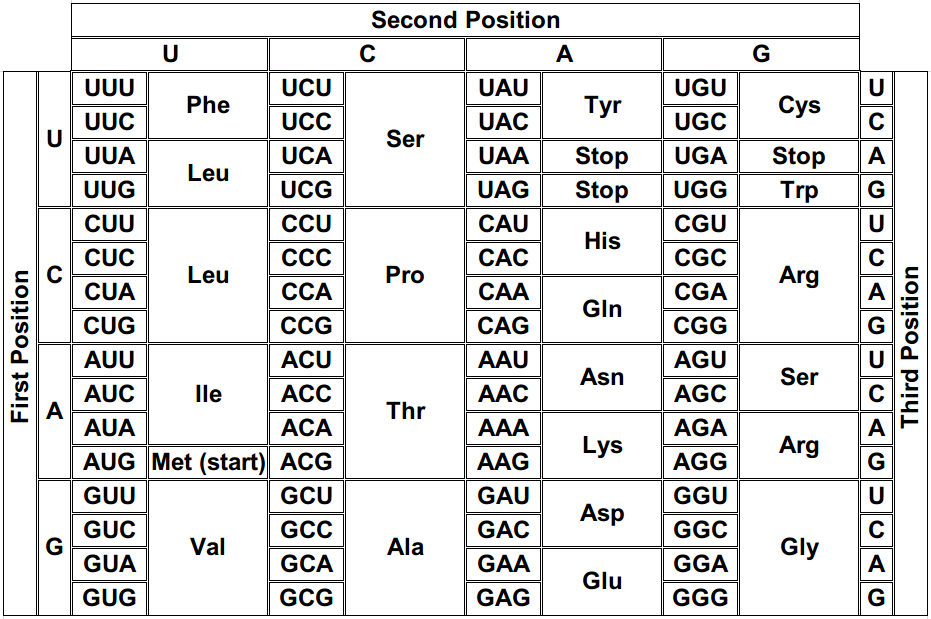
\includegraphics[width=15cm]{figure8.1.png}
  \caption{遗传密码}
  \label{fig:figure8.1}
\end{figure}

细胞中的翻译机器实际上会从RNA的某处起始,并“读取”一个接一个的密码子,把编码的氨基酸附加到不断增长的蛋白质序列的尾部。\autoref{exam:example8.1}模拟了这个过程,一次读取DNA字符串的三个碱基,然后把编码的氨基酸符号串联到不断增长的蛋白质字符串的尾部。在细胞中,当遇到三个终止密码子中的任意一个时,这个过程就会停止。

\subsection{把密码子翻译成氨基酸}
第一个任务,就是让后面的程序实现翻译的过程,就是把三个核苷酸的密码子翻译成氨基酸。对于研究三个核苷酸密码子编码一个氨基酸的遗传密码来说,这是最重要的一步。

下面是一个子程序,在给定三字母的DNA密码子后,它会返回一个(以单字母缩写表示的)氨基酸:

\begin{lstlisting}
# codon2aa
#
# A subroutine to translate a DNA 3-character codon to an amino acid

sub codon2aa {
  my($codon) = @_;
   
     if ( $codon =~ /TCA/i )   { return 'S' }   # Serine
  elsif ( $codon =~ /TCC/i )   { return 'S' }   # Serine
  elsif ( $codon =~ /TCG/i )   { return 'S' }   # Serine
  elsif ( $codon =~ /TCT/i )   { return 'S' }   # Serine
  elsif ( $codon =~ /TTC/i )   { return 'F' }   # Phenylalanine
  elsif ( $codon =~ /TTT/i )   { return 'F' }   # Phenylalanine
  elsif ( $codon =~ /TTA/i )   { return 'L' }   # Leucine
  elsif ( $codon =~ /TTG/i )   { return 'L' }   # Leucine
  elsif ( $codon =~ /TAC/i )   { return 'Y' }   # Tyrosine
  elsif ( $codon =~ /TAT/i )   { return 'Y' }   # Tyrosine
  elsif ( $codon =~ /TAA/i )   { return '_' }   # Stop
  elsif ( $codon =~ /TAG/i )   { return '_' }   # Stop
  elsif ( $codon =~ /TGC/i )   { return 'C' }   # Cysteine
  elsif ( $codon =~ /TGT/i )   { return 'C' }   # Cysteine
  elsif ( $codon =~ /TGA/i )   { return '_' }   # Stop
  elsif ( $codon =~ /TGG/i )   { return 'W' }   # Tryptophan
  elsif ( $codon =~ /CTA/i )   { return 'L' }   # Leucine
  elsif ( $codon =~ /CTC/i )   { return 'L' }   # Leucine
  elsif ( $codon =~ /CTG/i )   { return 'L' }   # Leucine
  elsif ( $codon =~ /CTT/i )   { return 'L' }   # Leucine
  elsif ( $codon =~ /CCA/i )   { return 'P' }   # Proline
  elsif ( $codon =~ /CCC/i )   { return 'P' }   # Proline
  elsif ( $codon =~ /CCG/i )   { return 'P' }   # Proline
  elsif ( $codon =~ /CCT/i )   { return 'P' }   # Proline
  elsif ( $codon =~ /CAC/i )   { return 'H' }   # Histidine
  elsif ( $codon =~ /CAT/i )   { return 'H' }   # Histidine
  elsif ( $codon =~ /CAA/i )   { return 'Q' }   # Glutamine
  elsif ( $codon =~ /CAG/i )   { return 'Q' }   # Glutamine
  elsif ( $codon =~ /CGA/i )   { return 'R' }   # Arginine
  elsif ( $codon =~ /CGC/i )   { return 'R' }   # Arginine
  elsif ( $codon =~ /CGG/i )   { return 'R' }   # Arginine
  elsif ( $codon =~ /CGT/i )   { return 'R' }   # Arginine
  elsif ( $codon =~ /ATA/i )   { return 'I' }   # Isoleucine
  elsif ( $codon =~ /ATC/i )   { return 'I' }   # Isoleucine
  elsif ( $codon =~ /ATT/i )   { return 'I' }   # Isoleucine
  elsif ( $codon =~ /ATG/i )   { return 'M' }   # Methionine
  elsif ( $codon =~ /ACA/i )   { return 'T' }   # Threonine
  elsif ( $codon =~ /ACC/i )   { return 'T' }   # Threonine
  elsif ( $codon =~ /ACG/i )   { return 'T' }   # Threonine
  elsif ( $codon =~ /ACT/i )   { return 'T' }   # Threonine
  elsif ( $codon =~ /AAC/i )   { return 'N' }   # Asparagine
  elsif ( $codon =~ /AAT/i )   { return 'N' }   # Asparagine
  elsif ( $codon =~ /AAA/i )   { return 'K' }   # Lysine
  elsif ( $codon =~ /AAG/i )   { return 'K' }   # Lysine
  elsif ( $codon =~ /AGC/i )   { return 'S' }   # Serine
  elsif ( $codon =~ /AGT/i )   { return 'S' }   # Serine
  elsif ( $codon =~ /AGA/i )   { return 'R' }   # Arginine
  elsif ( $codon =~ /AGG/i )   { return 'R' }   # Arginine
  elsif ( $codon =~ /GTA/i )   { return 'V' }   # Valine
  elsif ( $codon =~ /GTC/i )   { return 'V' }   # Valine
  elsif ( $codon =~ /GTG/i )   { return 'V' }   # Valine
  elsif ( $codon =~ /GTT/i )   { return 'V' }   # Valine
  elsif ( $codon =~ /GCA/i )   { return 'A' }   # Alanine
  elsif ( $codon =~ /GCC/i )   { return 'A' }   # Alanine
  elsif ( $codon =~ /GCG/i )   { return 'A' }   # Alanine
  elsif ( $codon =~ /GCT/i )   { return 'A' }   # Alanine
  elsif ( $codon =~ /GAC/i )   { return 'D' }   # Aspartic Acid
  elsif ( $codon =~ /GAT/i )   { return 'D' }   # Aspartic Acid
  elsif ( $codon =~ /GAA/i )   { return 'E' }   # Glutamic Acid
  elsif ( $codon =~ /GAG/i )   { return 'E' }   # Glutamic Acid
  elsif ( $codon =~ /GGA/i )   { return 'G' }   # Glycine
  elsif ( $codon =~ /GGC/i )   { return 'G' }   # Glycine
  elsif ( $codon =~ /GGG/i )   { return 'G' }   # Glycine
  elsif ( $codon =~ /GGT/i )   { return 'G' }   # Glycine
  else {
    print STDERR "Bad codon \"$codon\"!!\n";
    exit;
  }
}
\end{lstlisting}

这个代码非常清晰、简单,其排版布局也使得整个过程一目了然。然后,它运行起来却要耗费一定的时间。比如,对于代表甘氨酸的密码子GGT,它需要一个一个的进行测试,直到到达最后一行才会测试成功,这是一个大量的字符串比较。但不管怎么说,这些代码实现了最终的目的。

在代码中关于错误信息的部分出现了一些新的东西。回忆一下\autoref{chap:chapter4}中的文件句柄,以及它们是如何访问文件中的数据的。在\autoref{chap:chapter5}中,我们提到STDIN这个特殊的文件句柄会从键盘上读取用户的输入。STDOUT和STDERR也是特殊的文件句柄,在Perl程序中你总是可以使用它们。STDOUT把输出定向到屏幕(通常情况下)或者其他标准的输出位置。在 \verb|print|语句中没有指定文件句柄的时候,默认就会使用STDOUT。\textit{print}语句可以使用一个文件句柄作为可选的参数,但到目前为止,我们都把结果直接打印到了默认的STDOUT。在这个例子中,错误信息被定向到了STDERR,通常情况下就是被打印到屏幕,但在许多计算机系统中,它们可以被定向到一个特定的错误文件或者其他地方。另外,有时你会想把STDOUT定向到一个文件或者其他地方,而让STDERR错误信息显示在你的屏幕上。我之所以提到这些选项,是因为你很可能会在Perl代码中碰到它们,但在本书中我们不会过多地使用它们(更多内容请参看\autoref{chap:chapterab})。

\subsection{遗传密码的冗余性}
我已经提到过遗传密码的冗余性,而刚才的子程序也清晰的展示了这种冗余性。能够在你的子程序中将这种冗余性表现的淋漓尽致,这可能比较有趣。注意这些具有冗余性的密码子的前两个碱基通常都是一样的,只有第三个碱基发生了变化。在正则表达式中你已经使用过字符集,可以来匹配任意的一个字符集合。现在,让我们尝试把子程序重写一下,对每一个冗余的密码子组都只进行一次测试:

\begin{lstlisting}
# codon2aa
#
# A subroutine to translate a DNA 3-character codon to an amino acid
#   Version 2

sub codon2aa {
  my($codon) = @_;
 
     if ( $codon =~ /GC./i)        { return 'A' }   # Alanine
  elsif ( $codon =~ /TG[TC]/i)     { return 'C' }   # Cysteine
  elsif ( $codon =~ /GA[TC]/i)     { return 'D' }   # Aspartic Acid
  elsif ( $codon =~ /GA[AG]/i)     { return 'E' }   # Glutamic Acid
  elsif ( $codon =~ /TT[TC]/i)     { return 'F' }   # Phenylalanine
  elsif ( $codon =~ /GG./i)        { return 'G' }   # Glycine
  elsif ( $codon =~ /CA[TC]/i)     { return 'H' }   # Histidine
  elsif ( $codon =~ /AT[TCA]/i)    { return 'I' }   # Isoleucine
  elsif ( $codon =~ /AA[AG]/i)     { return 'K' }   # Lysine
  elsif ( $codon =~ /TT[AG]|CT./i) { return 'L' }   # Leucine
  elsif ( $codon =~ /ATG/i)        { return 'M' }   # Methionine
  elsif ( $codon =~ /AA[TC]/i)     { return 'N' }   # Asparagine
  elsif ( $codon =~ /CC./i)        { return 'P' }   # Proline
  elsif ( $codon =~ /CA[AG]/i)     { return 'Q' }   # Glutamine
  elsif ( $codon =~ /CG.|AG[AG]/i) { return 'R' }   # Arginine
  elsif ( $codon =~ /TC.|AG[TC]/i) { return 'S' }   # Serine
  elsif ( $codon =~ /AC./i)        { return 'T' }   # Threonine
  elsif ( $codon =~ /GT./i)        { return 'V' }   # Valine
  elsif ( $codon =~ /TGG/i)        { return 'W' }   # Tryptophan
  elsif ( $codon =~ /TA[TC]/i)     { return 'Y' }   # Tyrosine
  elsif ( $codon =~ /TA[AG]|TGA/i) { return '_' }   # Stop
  else {
    print STDERR "Bad codon \"$codon\"!!\n";
    exit;
  }
}
\end{lstlisting}

使用字符集和正则表达式,现在的代码清晰的展示了遗传密码的冗余性。此外,还要注意,现在表示氨基酸的单字母代码已经是按照字母顺序排列的了。

像 \verb|[TC]|的字符集匹配一个单字符,匹配T或者匹配C。 \verb|.|是一个正则表达式,它匹配除换行符以外的任意字符。代表缬氨酸的 \verb|/GT./i|表达式匹配GTA、GTC、GTG和GTT,所有这些密码子编码的都是缬氨酸。(当然,点号匹配任意其他字符,但是我们假设的是 \verb|$codon|只包含A、C、G和T四个字符。)正则表达式后面的i表示既匹配大写字母,也匹配小写字母,比如 \verb|/T/i|就匹配T或者t。

这些正则表达式中一个新的特性就是使用了竖线或者管道(|)来分隔两种匹配选择。因此,对于丝氨酸来说, \verb=/TC.|AG[TC]/=匹配的是 \verb|/TC./|或者 \verb|/AG[TC]/|。在这个程序中,对于每一个正则表达式来说你仅仅需要两种选择,但你可以自己的喜好和需要使用尽可能多的竖线。

你也可以用小括号把正则表达式的一部分进行分组,并在其中使用竖线。举个例子, \verb=/give me a (break|meal)/=能匹配“give me a break”或者“give me a meal”。

\subsection{使用散列表示遗传密码}
如果你考虑使用散列来完成这个翻译过程,你会看到这才是比较自然的方法。对于每一个密码子键,都有一个氨基酸值相对应。下面是代码:

\begin{lstlisting}
#
# codon2aa
#
# A subroutine to translate a DNA 3-character codon to an amino acid
#   Version 3, using hash lookup

sub codon2aa {
  my($codon) = @_;

  $codon = uc $codon;
 
  my(%genetic_code) = (
  
  'TCA' => 'S',    # Serine
  'TCC' => 'S',    # Serine
  'TCG' => 'S',    # Serine
  'TCT' => 'S',    # Serine
  'TTC' => 'F',    # Phenylalanine
  'TTT' => 'F',    # Phenylalanine
  'TTA' => 'L',    # Leucine
  'TTG' => 'L',    # Leucine
  'TAC' => 'Y',    # Tyrosine
  'TAT' => 'Y',    # Tyrosine
  'TAA' => '_',    # Stop
  'TAG' => '_',    # Stop
  'TGC' => 'C',    # Cysteine
  'TGT' => 'C',    # Cysteine
  'TGA' => '_',    # Stop
  'TGG' => 'W',    # Tryptophan
  'CTA' => 'L',    # Leucine
  'CTC' => 'L',    # Leucine
  'CTG' => 'L',    # Leucine
  'CTT' => 'L',    # Leucine
  'CCA' => 'P',    # Proline
  'CCC' => 'P',    # Proline
  'CCG' => 'P',    # Proline
  'CCT' => 'P',    # Proline
  'CAC' => 'H',    # Histidine
  'CAT' => 'H',    # Histidine
  'CAA' => 'Q',    # Glutamine
  'CAG' => 'Q',    # Glutamine
  'CGA' => 'R',    # Arginine
  'CGC' => 'R',    # Arginine
  'CGG' => 'R',    # Arginine
  'CGT' => 'R',    # Arginine
  'ATA' => 'I',    # Isoleucine
  'ATC' => 'I',    # Isoleucine
  'ATT' => 'I',    # Isoleucine
  'ATG' => 'M',    # Methionine
  'ACA' => 'T',    # Threonine
  'ACC' => 'T',    # Threonine
  'ACG' => 'T',    # Threonine
  'ACT' => 'T',    # Threonine
  'AAC' => 'N',    # Asparagine
  'AAT' => 'N',    # Asparagine
  'AAA' => 'K',    # Lysine
  'AAG' => 'K',    # Lysine
  'AGC' => 'S',    # Serine
  'AGT' => 'S',    # Serine
  'AGA' => 'R',    # Arginine
  'AGG' => 'R',    # Arginine
  'GTA' => 'V',    # Valine
  'GTC' => 'V',    # Valine
  'GTG' => 'V',    # Valine
  'GTT' => 'V',    # Valine
  'GCA' => 'A',    # Alanine
  'GCC' => 'A',    # Alanine
  'GCG' => 'A',    # Alanine
  'GCT' => 'A',    # Alanine
  'GAC' => 'D',    # Aspartic Acid
  'GAT' => 'D',    # Aspartic Acid
  'GAA' => 'E',    # Glutamic Acid
  'GAG' => 'E',    # Glutamic Acid
  'GGA' => 'G',    # Glycine
  'GGC' => 'G',    # Glycine
  'GGG' => 'G',    # Glycine
  'GGT' => 'G',    # Glycine
  );

  if(exists $genetic_code{$codon}) {
    return $genetic_code{$codon};
  }else{
    print STDERR "Bad codon \"$codon\"!!\n";
    exit;
  }
}
\end{lstlisting}

子程序非常简单:它先初始化了一个散列,然后对散列中单个的参数依次进行查找。散列有64个键,每一个键都代表一个密码子。

注意,有\textit{exists}这样一个函数,如果散列中存在 \verb|$codon|这个键,他就会返回 \verb|true|。它的作用和\textit{codon2aa}子程序前两个版本中的\textit{else}语句完全一样。\footnote{在散列中,一个键可能存在,但它的值可能是未定义的。\textit{defined}函数能检查值是不是已经被定义了。另外,当然,值也可能是0或者空字符串,在这种情况下,像 \verb|if ($hash{$key})|这样的测试会失败,因为,即使键存在而且值也被定义了,但在条件测试中,这样的值会被测试为 \verb|false|。}

另外,还要注意,为了让子程序既可以处理大写字母也可以处理小写字母,你把输入的参数都转换成了大写字母,这样就可以和 \verb|%genetic_code|散列中的数据进行比较了。你不能把正则表达式作为散列的键,它必须是简单的标量值,比如一个字符串或者一个数字,所以必须首先进行大小写的转换。(还有一种选择,你可以让散列的大小翻倍。)类似的,也不能把字符集作为散列的键,所以对于64个密码子你都必须单个进行指定。

你可能会想为什么要费事的把代码中最后的那一部分放在子程序中呢,为什么不仅仅声明并初始化散列、然后不需要进入子程序而是直接对散列进行查询呢?好吧,实际上子程序还对不存在的键进行了一点错误检查,这样在你使用散列的时候,就不用每次都自己进行错误检查了,因为子程序已经帮你做了。

另外,把这部分代码放在子程序中,也是为未来考虑的一点保险措施。使用我们的子程序,你编写的代码只需要负责密码子的翻译即可,这样就可以很方便的转换为另一种进行翻译的方式。也许在将来Perl会添加进一种新的数据类型,也有可能你想从数据库或者DBM文件中进行查询。这样,你需要做的仅仅是修改子程序的内部代码而已。只要对子程序的接口界面保持不变——也就是说,只要它还是把一个密码子作为参数并返回一个单字母表示的氨基酸——在程序的其他部分你就不需要担心它是如何实现翻译的了。我们的子程序成了一个\textit{黑盒子}。这是使用子程序对程序进行模块化和组织的一个非常显著的优势。

之所以使用子程序表示遗传密码,还有一个好的生物学上的原因。事实上,因为对于哺乳动物、植物、昆虫和酵母来说,DNA编码氨基酸的方式都有所不同,对于线粒体来说更是如此,所以有不止一种遗传密码。因此如果你对遗传密码进行了模块化,你只需要对程序进行简单的修改就可以适用于一系列的物种了。

散列的另一优势是它非常快。不幸的是,我们的子程序在每次被调用时都要声明整个散列,即使是仅进行一次查询也是如此。这并不高效,事实上,它还有些慢。还有其他更加快速的方法,可以把遗传密码散列作为全局变量只声明一次,但这对于现在的我们来说还有点遥不可及。我们现在这个版本的优势在于它非常易读。所以,让我们对这个散列版本的\textit{codon2aa}感到心满意足,并把它放到\textit{BeginPerlBioinfo.pm}文件(参看\autoref{chap:chapter6})的模块中吧。

现在我们已经找到一个比较满意的方法,把密码子翻译成了氨基酸,在接下来的小节和例子中我们将会使用它。

\section{把DNA翻译成蛋白质}
\autoref{exam:example8.1}展示了新的\textit{codon2aa}子程序如何把一整个DNA序列翻译成蛋白质。

%\textbf{例8-1:把DNA翻译成蛋白质}
\lstinputlisting[label=exam:example8.1,caption={例8.1:把DNA翻译成蛋白质}]{./scripts/example8-1.pl}

就像在\autoref{chap:chapter6}中讨论的那样,要使它能正常工作,你需要把提供子程序的\textit{BeginPerlBioinfo.pm}模块放到一个程序可以找到的单独的文件中。你还需要把\textit{codon2aa}子程序添加到这个文件中。还有一种办法,你可以直接把子程序\textit{condon2aa}的代码添加到\autoref{exam:example8.1}中的程序中,然后移除对\textit{BeginPerlBioinfo.pm}模块的引用。

下面是\autoref{exam:example8.1}的输出:

\begin{lstlisting}
I translated the DNA

CGACGTCTTCGTACGGGACTAGCTCGTGTCGGTCGC

  into the protein

RRLRTGLARVGR
\end{lstlisting}

\autoref{exam:example8.1}中的所有元素你都已经在前面见到过了,除了循环遍历DNA的方法,就是下面这个语句:

\begin{lstlisting}
for(my $i=0; $i < (length($dna) - 2); $i += 3) {
\end{lstlisting}

回忆一下, \verb|for|由用两个分号隔开的三部分组成。第一部分初始化一个计数器: \verb|my $i=0|静态限定了 \verb|$i|变量的范围,这样它就只能在代码块中被使用了,而代码中其他部分出现的其他 \verb|$i|(好吧,在这个例子中,并没有其他这样的变量,但确实可能会出现这种情况)现在在代码块中则是不可用的。 \verb|for|循环的第三部分会在代码块中的所有语句执行完后、重新回到循环顶部前增加计数器。

\begin{lstlisting}
$i += 3
\end{lstlisting}

因为在遍历DNA时每次要处理三个碱基,所以你把计数器增加三。

 \verb|for|循环中间的第二部分测试判断是否要继续循环:

\begin{lstlisting}
$i < (length($dna) - 2)
\end{lstlisting}

关键点在于,如果有两个、一个或者没有碱基剩余时,你应该退出程序,因为它们不足以构成一个密码子了。现在,对于一个特定长度的DNA字符串来说,碱基位置的计数就是从 \verb|0|到 \verb|length-1|。所以如果位置计数器 \verb|$i|增加到了 \verb|length-2|,就只剩余两个碱基( \verb|length-2|和 \verb|length-1|位置处的碱基)了,这时你应该退出程序。当位置计数器 \verb|$i|小于 \verb|length-2|时,剩余的碱基至少还有三个,这足以构成一个密码子了。所以要想测试成功,只能:

\begin{lstlisting}
$i < (length($dna) - 2)
\end{lstlisting}

(注意一下,小于号后面的表达式是如何被包裹在小括号中的;我们将在\autoref{chap:chapter9}的\autoref{sect:section9.3.1}中对其进行讨论。)

这行代码:

\begin{lstlisting}
$codon = substr ($dna, $i 3);
\end{lstlisting}

实际上从DNA中提取了三碱基的密码子。通过调用 \verb|substr|函数,提取出 \verb|$dna|字符串上位置 \verb|$i|处长度为 \verb|3|的子字符串,并把它保存到了变量 \verb|$codon|中。

如果你知道,你需要进行很多从DNA到蛋白质的翻译,你可以把\autoref{exam:example8.1}转换成一个子程序。当你编写一个子程序时,你需要考虑你想把那些参数传递给子程序。所以你意识到,早晚有一天会遇到这样的情况,你有一些很长的DNA序列,但却只想翻译整个序列中指定的一部分。你是否应该给子程序添加两个参数来指定起始和终止位点呢?你可以这么做,但你决定先不这么做。这是一种主观判断——把代码集合分解成有用片段的艺术的一部分。但是最好有一个只负责翻译过程的子程序,然后,如果有需要,你可以把它作为从序列中选择终点的更大的子程序的一部分。此处的考虑是,你通常仅仅需要把整条序列都进行翻译,所以每次都键入 \verb|0|作为起始点、 \verb|length($dna)-1|作为终止点可能会让人厌烦。当然,这取决于你手头的工作,所以此处的选择仅供你在编写代码时思考之用。

你应该移除末尾输出信息的 \verb|print|语句,因为与子程序相比,它更加适合于主程序。

不管怎样,你已经思考了整个设计思路,现在只需要一个子程序,它需要一个包含DNA的参数,并返回翻译后的肽链:

\begin{lstlisting}
# dna2peptide 
#
# A subroutine to translate DNA sequence into a peptide

sub dna2peptide {
  
  my($dna) = @_;

  use strict;
  use warnings;
  use BeginPerlBioinfo;     # see Chapter 6 about this module

  # Initialize variables
  my $protein = '';

  # Translate each three-base codon to an amino acid, and append to a protein 
  for(my $i=0; $i < (length($dna) - 2) ; $i += 3) {
    $protein .= codon2aa( substr($dna,$i,3));
  }

  return $protein;
  }
\end{lstlisting}

现在把子程序\textit{dna2peptide}添加到\textit{BeginPerlBioinfo.pm}模块中吧。

注意,在你把\autoref{exam:example8.1}转换成子程序时,删除了一个变量:变量 \verb|$codon|。为什么呢?

好吧,一个原因就是你可以把它删除。在\autoref{exam:example8.1}中,你使用\textit{substr}从 \verb|$dna|中提取密码子,把它保存到变量 \verb|$codon|中,然后传递到子程序\textit{codon2aa}中。新的方法删除这个中间人。直接把提取密码子的对\textit{substr}的调用作为参数传递给子程序\textit{codon2aa},这样值像以前一样传递了进去,但却没有必要先把它复制到变量 \verb|$codon|中去了。

这在某种程度上提高了效率和速度。因为复制字符串是计算机程序做的非常慢的一件事情,删除一大批字符串的复制,是提高程序运行速度一种简单、有效的方法。

但是这有没有削弱程序的易读性呢?这由你来判断。我觉得有那么一点,但是对于我来说,无论如何,循环前面的注释看起来已经让一切都清晰明了了。编写易读的代码非常重要,所以如果你确实需要大幅提升子程序的速度,但却发现使代码更加难读了,一定要确保包含足够的注释,让读者可以理解所发生的一切。

\textit{use}函数的调用第一次被包含在了子程序中而不是主程序中:

\begin{lstlisting}
use strict;
use warnings;
use BeginPerlBioinfo;
\end{lstlisting}

这可能和主程序中的调用存在冗余,但这并没有任何坏处(Perl会进行检查,并且只载入模块一次)。如果在一个没有载入这些模块的模块中调用这个子程序,它还是可以正常工作。

现在,让我们来看看如何处理文件中的DNA。

\section{从文件中读取FASTA格式的DNA}
在生物信息学短暂的历史中,许多不同的生物学家和程序员发明了各种在计算机文件中格式化序列数据的方法,导致生物信息学家不得不去处理这些不同的格式。我们需要从这些文件中提取出序列数据和注释信息,对于每种不同的格式,这都需要编写代码进行处理。

有许多这样的格式,仅仅针对DNA的常用格式可能就有20种之多。当你在实验室中分析序列时,格式的这种多样化会让人头疼不已:因为对于你用来分析序列的各种程序,都需要把一种格式转换成另一种格式。下面是几个最流行的格式:

\textcolor{red}{\textit{FASTA}}
\begin{adjustwidth}{4em}{}
FASTA和基本局部相似性比对搜索技术(BLAST\footnote{译者注:BLAST是Basic Local Alignment Search Tool的缩写。},Basic Local Alignment Search Technique)程序非常流行,它们都使用FASTA格式。因为它的简洁性,FASTA格式可能是所有格式中除GenBank格式以外使用最为广泛的一种格式。
\end{adjustwidth}

\textcolor{red}{\textit{Genetic Sequence Data Bank (GenBank\footnote{译者注:GenBank指的是Genetic Sequence Database。})}}
\begin{adjustwidth}{4em}{}
GenBank收集了所有公开发表的遗传数据。除了DNA序列,它还包括了许多相关的信息。它非常重要,所以我们将在\autoref{chap:chapter10}中对GenBank文件进行深入探讨。
\end{adjustwidth}

\textcolor{red}{\textit{欧洲分子生物学实验室(EMBL,European Molecular Biology Laboratory)}}
\begin{adjustwidth}{4em}{}
EMBL数据库大体上和GenBank、DDBJ(日本DNA数据库,DNA Data Bank of Japan)存储有相同的数据,但格式稍有不同。
\end{adjustwidth}

\textcolor{red}{\textit{简单数据,或美国应用生物系统公司(ABI,Applied Biosystems)测序仪的输出}}
\begin{adjustwidth}{4em}{}
这是没有进行任何格式化的DNA序列数据,仅仅是代表碱基的字符而已。ABI的测序机器和其他机器以及程序把它直接输出到文件中。
\end{adjustwidth}

\textcolor{red}{\textit{蛋白质识别资源(PIR,Protein Identification Resource)}}
\begin{adjustwidth}{4em}{}
PIR是一个良好组织的蛋白质序列数据集合。
\end{adjustwidth}

\textcolor{red}{\textit{遗传学电脑集团(GCG,Genetics Computer Group)}}
\begin{adjustwidth}{4em}{}
Accelrys的GCG程序(亦称GCG Wisconsin
package)在许多大型研究机构中使用。要想被它们的程序使用,数据必须以GCG格式进行存储。
\end{adjustwidth}

在这六种序列格式中,GenBank和FASTA是迄今为止最常用的格式。接下来的几个小节将向你介绍FASTA格式数据的读取和处理过程。

\subsection{FASTA格式}
让我们编写一个子程序,来处理FASTA格式的数据。它本身就非常有用,而且可以作为后续章节处理GenBank、PDB和BLAST的热身。

FASTA格式基本上就是序列数据行,在其末尾有换行符,这样就可以把它打印到纸上或者显示在计算机屏幕上。行的长度没有特别指定,但是为了兼容,最好把长度限制在80个字符以内。此外,还有一个\textit{头信息},就是文件开头以大于号>起始的一行或数行,它可以包含任意文字(或者没有文字)。通常,标题行包括DNA或者它的来源基因的名字,一般用竖线将其和序列的其他信息、生成它的实验或者其他类似的非序列的信息分隔开来。

许多使用FASTA格式的软件都坚持认为只能有一行头信息,其他则允许多行头信息的存在。我们的子程序对一行或多行头信息以及以\#起始的注释都能够进行处理。

下面是一个FASTA文件。我们把它叫做\textit{sample.dna},并且在许多程序中都将使用到它。你应该从书籍网站上复制、下载它,或者用你自己的数据制作出自己的文件。

\begin{lstlisting}
> sample dna | (This is a typical fasta header.)
agatggcggcgctgaggggtcttgggggctctaggccggccacctactgg
tttgcagcggagacgacgcatggggcctgcgcaataggagtacgctgcct
gggaggcgtgactagaagcggaagtagttgtgggcgcctttgcaaccgcc
tgggacgccgccgagtggtctgtgcaggttcgcgggtcgctggcgggggt
cgtgagggagtgcgccgggagcggagatatggagggagatggttcagacc
cagagcctccagatgccggggaggacagcaagtccgagaatggggagaat
gcgcccatctactgcatctgccgcaaaccggacatcaactgcttcatgat
cgggtgtgacaactgcaatgagtggttccatggggactgcatccggatca
ctgagaagatggccaaggccatccgggagtggtactgtcgggagtgcaga
gagaaagaccccaagctagagattcgctatcggcacaagaagtcacggga
gcgggatggcaatgagcgggacagcagtgagccccgggatgagggtggag
ggcgcaagaggcctgtccctgatccagacctgcagcgccgggcagggtca
gggacaggggttggggccatgcttgctcggggctctgcttcgccccacaa
atcctctccgcagcccttggtggccacacccagccagcatcaccagcagc
agcagcagcagatcaaacggtcagcccgcatgtgtggtgagtgtgaggca
tgtcggcgcactgaggactgtggtcactgtgatttctgtcgggacatgaa
gaagttcgggggccccaacaagatccggcagaagtgccggctgcgccagt
gccagctgcgggcccgggaatcgtacaagtacttcccttcctcgctctca
ccagtgacgccctcagagtccctgccaaggccccgccggccactgcccac
ccaacagcagccacagccatcacagaagttagggcgcatccgtgaagatg
agggggcagtggcgtcatcaacagtcaaggagcctcctgaggctacagcc
acacctgagccactctcagatgaggaccta
\end{lstlisting}

\subsection{读取FASTA文件的设计}
在\autoref{chap:chapter4}中,你学习了如何读入序列数据。此处,你只需要将其进行扩展以便能够处理标题行。你还将学习到如何丢弃空行以及以井号(磅字符)\#起始的行,也就是Perl和其他语言以及文件格式中的注释。(这样的行在刚刚展示的FASTA文件\textit{sample.dna}中并没有出现。)

当读入数据时有两种选择。你可以从打开的文件中一次读入一行,随读入随进行处理。或者,你也可以一次性把整个文件都读入到数组中,然后对数组进行操作。对于非常大的文件来说,尤其是你寻找一些小的信息片段时,最好一次只读入文件的一行。(这是因为把一个大的文件读入数组会占用大量的内存空间。如果你的计算机不够强大,可能会导致系统崩溃。)

对于小的、正常大小的文件来说,把所有数据读入数组的好处在于,之后你可以轻松地遍历数据对它进行操作。这就是我们的子程序所做的事情,但是一定要记住,对于大文件来说这种方法可能会导致内存空间问题,还有其他的方法可以采用。

让我们编写一个子程序,给定一个包含FASTA格式数据的文件名参数,它会返回序列数据。

在动手之前,你应该考虑你是否只需要一个子程序,还是一个子程序打开并读取文件、另一个子程序调用它并提取序列数据。我们使用两个子程序,一定要牢记在心,每次当你需要编写类似的程序处理其他格式时,你都可以重用这里处理任意文件的子程序。

我们由伪代码开始:

\begin{lstlisting}
subroutine get data from a file

  argument = filename

  open file
    if can't open, print error message and exit

  read in data and 

  return @data
}

Subroutine extract sequence data from fasta file

  argument = array of file data in fasta format

    Discard all header lines
    (and blank and comment lines for good measure)
    If first character of first line is >, discard it

  Read in the rest of the file, join in a scalar,
    edit out nonsequence data

  return sequence
}
\end{lstlisting}

在第一个从文件中获取数据的子程序中,存在这样一个问题,当文件不能被读取时,最好的处理办法是什么。此处,我们采用了最极端的方案:尖叫“着火了!”然后跳出。但是你可能不一定想让你的程序在无法打开文件时立即停止。也许,你想通过键盘或者网页向用户询问文件名,并给他们三次机会来键入正确的文件名。又或者,如果文件无法打开,你就使用默认的文件进行替代。

当你无法打开文件时,也许你可以返回 \verb|false|值,比如一个空数组。然后,调用这个子程序的程序就可以退出,重试,或者其他它想进行的操作。但是,如果你成功打开了文件,但却完全是空的呢?这时,你成功打开了文件,并返回一个空数组,而调用这个子程序的程序可能会错误的认为文件无法打开。所以,这种方案并不可取。

还有其他的选择,比如返回特殊的“未定义”值。我们还是言归正传,但牢记这么一点是非常重要的,处理错误很重要,有时非常晦涩,这也是编写\textit{强健代码}的一部分,这种代码可以很好的处理异常情况。

第二个子程序,处理存储FASTA格式序列的数组,并返回未格式化的序列字符串。

\subsection{读取FASTA文件的子程序}
既然你已经思考了问题、编写了伪代码、想到了设计子程序的不同方案以及不同选择的利弊,现在就可以真正开始编写代码了:

\begin{lstlisting}
# get_file_data
#
# A subroutine to get data from a file given its filename

sub get_file_data {

  my($filename) = @_;

  use strict;
  use warnings;

  # Initialize variables
  my @filedata = ( );

  unless( open(GET_FILE_DATA, $filename) ) {
    print STDERR "Cannot open file \"$filename\"\n\n";
    exit;
  }

  @filedata = <GET_FILE_DATA>;

  close GET_FILE_DATA;

  return @filedata;
}

# extract_sequence_from_fasta_data
#
# A subroutine to extract FASTA sequence data from an array

sub extract_sequence_from_fasta_data {

  my(@fasta_file_data) = @_;

  use strict;
  use warnings;

  # Declare and initialize variables
  my $sequence = '';

  foreach my $line (@fasta_file_data) {

    # discard blank line
    if ($line =~ /^\s*$/) {
      next;

    # discard comment line
    } elsif($line =~ /^\s*#/) {
      next;

    # discard fasta header line
    } elsif($line =~ /^>/) {
      next;

    # keep line, add to sequence string
    } else {
      $sequence .= $line;
    }
  }

  # remove non-sequence data (in this case, whitespace) from $sequence string
  $sequence =~ s/\s//g;

  return $sequence;
}
\end{lstlisting}

注意,在\textit{extract\_sequence\_from\_fasta\_data}的代码中你并没有检查文件中存储的内容:它是不是真的是以FASTA格式存储的DNA或者蛋白质序列?当然,你可以编写一个子程序——把它叫做\textit{is\_fasta}——来检查数据看看它是不是我们所期望的那样。但这里我把它留作课后练习。

对于\textit{extract\_sequence\_from\_fasta\_data}子程序要进行一些注释。下面这行代码包括一个在循环中使用的变量的声明。

\begin{lstlisting}
foreach my $line (@fasta_file_data) {
\end{lstlisting}

在 \verb|for|循环中你已经见过这样的情况。在使用 \verb|$line|的地方使用 \verb|my|对变量进行声明,这非常方便,因为它们往往都有比较常见的名字,而且在循环外不会被使用到。

一些正则表达式需要进行简要的注释。这一行代码:

\begin{lstlisting}
if ($line =~ /^\s*$/) {
\end{lstlisting}

其中, \verb|\s|匹配空白,也就是空格、制表符、换页符、回车符或者换行符。 \verb|\s*|匹配任意数量的空白(即使没有)。 \verb|^|匹配行首,而 \verb|$|则匹配行尾。所以综合起来,这个正则表达式匹配的是没有或者只有空白的空行。

这个正则表达式表示的是行首没有或者只有空白、之后紧跟井号:

\begin{lstlisting}
} elsif($line =~ /^\s*#/) {
\end{lstlisting}

这个正则表达式匹配的是行首的大于号:

\begin{lstlisting}
} elsif($line =~ /^>/) {
\end{lstlisting}

最后,下面这个语句删除空白,包括换行符:

\begin{lstlisting}
$sequence =~ s/\s//g;
\end{lstlisting}

我们已经把这两个新的子程序放到了我们的\textit{BeginPerlBioinfo.pm}模块中。现在,我们来为这些子程序编写一个主程序,看看它的输出。首先,还需要编写一个子程序,来处理长序列的输出。

\subsection{输出格式化的序列数据}
当你试图打印输出“原始的”序列数据时,如果数据长度远远超过纸张的宽度,会出现问题。实际上,如果你尝试让它适合纸张,80个字符大约是你应该使用的最大的长度。我们编写一个\textit{print\_sequence}子程序,它以一些序列和行的长度作为参数,把序列打断成要求长度的多行并打印输出出来。它和\textit{dna2peptide}子程序有很高的相似度。这是代码:

\begin{lstlisting}
# print_sequence
#
# A subroutine to format and print sequence data 

sub print_sequence {
  
  my($sequence, $length) = @_;

  use strict;
  use warnings;

  # Print sequence in lines of $length
  for ( my $pos = 0 ; $pos < length($sequence) ; $pos += $length  ) {
    print substr($sequence, $pos, $length), "\n";
  }
}
\end{lstlisting}

代码依赖于\textit{substr}的行为,它会在字符串后面输出部分子字符串,即使其长度小于要求的长度。你可以看到在\textit{BeginPerlBioinfo.pm}模块(参看\autoref{chap:chapter6})中出现了新的\textit{print\_sequence}子程序。记住,一定要把语句 \verb|1;|作为模块的最后一行。\autoref{exam:example8.2}演示的是主程序。

%\textbf{例8-2:读取FASTA文件并提取序列数据}
\lstinputlisting[label=exam:example8.2,caption={例8.2:读取FASTA文件并提取序列数据}]{./scripts/example8-2.pl}

下面是\autoref{exam:example8.2}的输出:

\begin{lstlisting}
agatggcggcgctgaggggtcttgg
gggctctaggccggccacctactgg
tttgcagcggagacgacgcatgggg
cctgcgcaataggagtacgctgcct
gggaggcgtgactagaagcggaagt
agttgtgggcgcctttgcaaccgcc
tgggacgccgccgagtggtctgtgc
aggttcgcgggtcgctggcgggggt
cgtgagggagtgcgccgggagcgga
gatatggagggagatggttcagacc
cagagcctccagatgccggggagga
cagcaagtccgagaatggggagaat
gcgcccatctactgcatctgccgca
aaccggacatcaactgcttcatgat
cgggtgtgacaactgcaatgagtgg
ttccatggggactgcatccggatca
ctgagaagatggccaaggccatccg
ggagtggtactgtcgggagtgcaga
gagaaagaccccaagctagagattc
gctatcggcacaagaagtcacggga
gcgggatggcaatgagcgggacagc
agtgagccccgggatgagggtggag
ggcgcaagaggcctgtccctgatcc
agacctgcagcgccgggcagggtca
gggacaggggttggggccatgcttg
ctcggggctctgcttcgccccacaa
atcctctccgcagcccttggtggcc
acacccagccagcatcaccagcagc
agcagcagcagatcaaacggtcagc
ccgcatgtgtggtgagtgtgaggca
tgtcggcgcactgaggactgtggtc
actgtgatttctgtcgggacatgaa
gaagttcgggggccccaacaagatc
cggcagaagtgccggctgcgccagt
gccagctgcgggcccgggaatcgta
caagtacttcccttcctcgctctca
ccagtgacgccctcagagtccctgc
caaggccccgccggccactgcccac
ccaacagcagccacagccatcacag
aagttagggcgcatccgtgaagatg
agggggcagtggcgtcatcaacagt
caaggagcctcctgaggctacagcc
acacctgagccactctcagatgagg
accta
\end{lstlisting}

\subsection{读入DNA输出蛋白质的主程序}
现在,这是本小节的最后一个程序。我们向上面的程序中添加从DNA到蛋白质的翻译过程,最后输出蛋白质而不是DNA。注意\autoref{exam:example8.3}是多么的精炼!随着你不断向我们的模块中积累有用的子程序,编写程序会越来越容易。

%\textbf{例8-3:读取DNA的FASTA文件,翻译成蛋白质,并格式化输出}
\lstinputlisting[label=exam:example8.3,caption={例8.3:读取DNA的FASTA文件,翻译成蛋白质,并格式化输出}]{./scripts/example8-3.pl}

下面是\autoref{exam:example8.3}的输出:

\begin{lstlisting}
RWRR_GVLGALGRPPTGLQRRRRMG
PAQ_EYAAWEA_LEAEVVVGAFATA
WDAAEWSVQVRGSLAGVVRECAGSG
DMEGDGSDPEPPDAGEDSKSENGEN
APIYCICRKPDINCFMIGCDNCNEW
FHGDCIRITEKMAKAIREWYCRECR
EKDPKLEIRYRHKKSRERDGNERDS
SEPRDEGGGRKRPVPDPDLQRRAGS
GTGVGAMLARGSASPHKSSPQPLVA
TPSQHHQQQQQQIKRSARMCGECEA
CRRTEDCGHCDFCRDMKKFGGPNKI
RQKCRLRQCQLRARESYKYFPSSLS
PVTPSESLPRPRRPLPTQQQPQPSQ
KLGRIREDEGAVASSTVKEPPEATA
TPEPLSDEDL
\end{lstlisting}

\section{阅读框}
生物学家都知道,给定一个DNA序列,需要检查这个DNA所有的六种\textit{阅读框},来寻找细胞用来编码蛋白质的编码区域。

\subsection{什么是阅读框?}
通常情况下你都不知道细胞实际上是从你研究的DNA的那个地方开始把它翻译成蛋白质的。只有大约1-1.5\%的人类DNA是基因\footnote{译者注:此段中的基因实际上指的是编码区,或者说是外显子。},也就是用来翻译成蛋白质的DNA片段。此外,基因通常都是以片段的形式存在,在转录/翻译的过程中它们会被剪切、拼接在一起。

如果你不知道翻译从何处起始,你就必须要考虑六种可能的阅读框。因为密码子长3个碱基,所以翻译可以发生在三个“框”内,比如从第一个碱基、第二个碱基或者第三个碱基开始。(从第四个碱基开始实际上是和从第一个碱基开始完全一样的。)每一种起始位置都会给出一系列不同的密码子,最终就是一系列不同的氨基酸。

此外,转录和翻译可以发生在DNA的两条链上,也就是DNA序列或者它的反向互补序列都可能包含最终被翻译的DNA编码。反向互补序列也可以从三种不同框的任意一种内进行阅读。所以,寻找编码区域、也就是编码蛋白质的DNA片段时,总共有六种阅读框需要考虑。

因此这非常常见,通过检查DNA序列的所有六种阅读框来寻找最终的蛋白质翻译,找到没有终止密码子的连续的长的氨基酸片段。

\textit{终止密码子}肯定会打断DNA$\rightarrow$protein的翻译过程。在翻译过程(实际上是从RNA到蛋白质,但是我故意模糊简化了生物化学)中,如果碰到一个终止密码子,翻译就会停止,不断增长的肽链也会停止增长。

不包含终止密码子的长的DNA片段叫做\textit{开放阅读框}(ORFs,open reading
frames),是判断正在研究的DNA中存在基因的一个重要的依据。所以基因识别程序需要进行这种阅读框的分析,这也正是我们在本章中学习的内容。

\subsection{翻译阅读框}
基于上述事实,我们编写一些代码,来把DNA进行六个阅读框的翻译。

在现实生活中,你可能会四处寻找已经写好的、可以完成该任务的子程序。基于任务的基本属性——研究DNA的工作者一定会做的事情——你很可能会找到这样的代码。但是这里是一个指南,而不是现实世界,所以还是让我们披挂上阵吧。

这个问题并没有听上去那么吓人。所以,检查一下你的子程序行囊,(利用手头可以使用的子程序储备,)想想你现在身处何方、该如何到达目的地。

查看一下我们已经编写的子程序,回想一下\textit{dna2peptide}。你可能会想到添加一些参数来指定起始和结束位点。现在就让我们动手吧。

还记得吗,尽管我们在\autoref{chap:chapter4}中计算了反向互补序列,但我们并没有把它编写成子程序。所以我们先从这里开始:

\begin{lstlisting}
# revcom 
#
# A subroutine to compute the reverse complement of DNA sequence

sub revcom {

  my($dna) = @_;

  # First reverse the sequence
  my($revcom) = reverse($dna);

  # Next, complement the sequence, dealing with upper and lower case
  # A->T, T->A, C->G, G->C
  $revcom =~ tr/ACGTacgt/TGCAtgca/;

  return $revcom;
}
\end{lstlisting}

现在,这是一点伪代码,展示将要翻译DNA特定区间的子程序的思路:

\begin{lstlisting}
Given DNA sequence

subroutine translate_frame ( DNA, start, end )

  return dna2peptide( substr( DNA, start, end - start + 1 ) )

}
\end{lstlisting}

这就很好!幸运的是,当把DNA传递进已经写好的\textit{dna2peptide}子程序中时,Perl的内置函数\textit{substr}使得它可以非常容易的使用指定的起始和终止位点。

注意序列的长度是 \verb|end-start+1|。考虑一个简单的例子:如果你从位置3起始、到位置5终止,你会得到位置3、4和5的碱基,总共有三个碱基,正好等于5 - 3 + 1。

处理类似这样的索引要非常小心,否则代码可能无法正常工作。对于许多程序来说,这是数学最讨人烦的地方。

%\begin{adjustwidth}{4em}{4em}
  %\parpic[l]{
  %
\includegraphics[width=1cm]{warning.png}
%}
%\noindent
%小心索引!
%\end{adjustwidth}

\vspace{-5pt}
\begin{table}[h]
  \begin{center}
    \begin{tabu} to 0.85\linewidth {|X[1,r,m]X[15,l,m]|}
      \tabucline{-}
      
\includegraphics[width=1.1cm]{warning.png} & 小心索引!\\
      \tabucline{-}
    \end{tabu}
  \end{center}
\end{table}
\vspace{-20pt}

你需要决定,你是要从0开始对位置进行计数,这是Perl的处理方式,还是把序列的第一个字符作为位置1,这是生物学家的处理方式。我们采用生物学家的处理方式。当传递给Perl的函数\textit{substr}时,位置要减一,当然,最终还是Perl的处理方式。

纠正后的伪代码是这样子的:

\begin{lstlisting}
Given DNA sequence

subroutine translate_frame ( DNA, start, end )

  # start and end are numbering the sequence from 1 to length

  return dna2peptide( substr( DNA, start - 1, end - start + 1 ) )
}
\end{lstlisting}

序列的长度并没有随索引的改变而改变,因为:

\begin{lstlisting}
(end - 1) - (start - 1) + 1 = end - start + 1
\end{lstlisting}

现在我们来编写这个子程序:

\begin{lstlisting}
# translate_frame
#
# A subroutine to translate a frame of DNA

sub translate_frame {

  my($seq, $start, $end) = @_;

  my $protein;

  # To make the subroutine easier to use, you won't need to specify
  #  the end point--it will just go to the end of the sequence
  #  by default.
  unless($end) {
    $end = length($seq);
  }

  # Finally, calculate and return the translation
    return dna2peptide ( substr ( $seq, $start - 1, $end -$start + 1 ) );
}
\end{lstlisting}

\autoref{exam:example8.4}从六个阅读框上翻译DNA。

%\textbf{例8-4:从六个阅读框上翻译DNA序列}
\lstinputlisting[label=exam:example8.4,caption={例8.4:从六个阅读框上翻译DNA序列}]{./scripts/example8-4.pl}

下面是\autoref{exam:example8.4}的输出:

\begin{lstlisting}
 -------Reading Frame 1--------

RWRR_GVLGALGRPPTGLQRRRRMGPAQ_EYAAWEA_LEAEVVVGAFATAWDAAEWSVQVRGSLAGVVRE
CAGSGDMEGDGSDPEPPDAGEDSKSENGENAPIYCICRKPDINCFMIGCDNCNEWFHGDCIRITEKMAKA
IREWYCRECREKDPKLEIRYRHKKSRERDGNERDSSEPRDEGGGRKRPVPDPDLQRRAGSGTGVGAMLAR
GSASPHKSSPQPLVATPSQHHQQQQQQIKRSARMCGECEACRRTEDCGHCDFCRDMKKFGGPNKIRQKCR
LRQCQLRARESYKYFPSSLSPVTPSESLPRPRRPLPTQQQPQPSQKLGRIREDEGAVASSTVKEPPEATA
TPEPLSDEDL

 -------Reading Frame 2--------

DGGAEGSWGL_AGHLLVCSGDDAWGLRNRSTLPGRRD_KRK_LWAPLQPPGTPPSGLCRFAGRWRGS_GS
APGAEIWREMVQTQSLQMPGRTASPRMGRMRPSTASAANRTSTAS_SGVTTAMSGSMGTASGSLRRWPRP
SGSGTVGSAERKTPS_RFAIGTRSHGSGMAMSGTAVSPGMRVEGARGLSLIQTCSAGQGQGQGLGPCLLG
ALLRPTNPLRSPWWPHPASITSSSSSRSNGQPACVVSVRHVGALRTVVTVISVGT_RSSGAPTRSGRSAG
CASASCGPGNRTSTSLPRSHQ_RPQSPCQGPAGHCPPNSSHSHHRS_GASVKMRGQWRHQQSRSLLRLQP
HLSHSQMRT

 -------Reading Frame 3--------

MAALRGLGGSRPATYWFAAETTHGACAIGVRCLGGVTRSGSSCGRLCNRLGRRRVVCAGSRVAGGGREGV
RRERRYGGRWFRPRASRCRGGQQVREWGECAHLLHLPQTGHQLLHDRV_QLQ_VVPWGLHPDH_EDGQGH
PGVVLSGVQRERPQARDSLSAQEVTGAGWQ_AGQQ_APG_GWRAQEACP_SRPAAPGRVRDRGWGHACSG
LCFAPQILSAALGGHTQPASPAAAAADQTVSPHVW_V_GMSAH_GLWSL_FLSGHEEVRGPQQDPAEVPA
APVPAAGPGIVQVLPFLALTSDALRVPAKAPPATAHPTAATAITEVRAHP_R_GGSGVINSQGAS_GYSH
T_ATLR_GP

 -------Reading Frame 4--------

_VLI_EWLRCGCSLRRLLDC_  _RHCPLIFTDAP_LL_WLWLLLGGQWPAGPWQGL_GRHW_ERGREVLVR
FPGPQLALAQPALLPDLVGAPELLHVPTEITVTTVLSAPTCLTLTTHAG_PFDLLLLLLVMLAGCGHQGL
RRGFVGRSRAPSKHGPNPCP_PCPALQVWIRDRPLAPSTLIPGLTAVPLIAIPLP_LLVPIANL_LGVFL
SALPTVPLPDGLGHLLSDPDAVPMEPLIAVVTPDHEAVDVRFAADAVDGRILPILGLAVLPGIWRLWV_T
ISLHISAPGALPHDPRQRPANLHRPLGGVPGGCKGAHNYFRF_SRLPGSVLLLRRPHASSPLQTSRWPA_
SPQDPSAPPS

 -------Reading Frame 5--------

RSSSESGSGVAVASGGSLTVDDATAPSSSRMRPNFCDGCGCCWVGSGRRGLGRDSEGVTGESEEGKYLYD
SRARSWHWRSRHFCRILLGPPNFFMSRQKSQ_PQSSVRRHASHSPHMRADRLICCCCCW_CWLGVATKGC
GEDLWGEAEPRASMAPTPVPDPARRCRSGSGTGLLRPPPSSRGSLLSRSLPSRSRDFLCR_RISSLGSFS
LHSRQYHSRMALAIFSVIRMQSPWNHSLQLSHPIMKQLMSGLRQMQ_MGAFSPFSDLLSSPASGGSGSEP
SPSISPLPAHSLTTPASDPRTCTDHSAASQAVAKAPTTTSASSHASQAAYSYCAGPMRRLRCKPVGGRPR
APKTPQRRH

 -------Reading Frame 6--------

GPHLRVAQVWL_PQEAP_LLMTPLPPHLHGCALTSVMAVAAVGWAVAGGALAGTLRASLVRARKGSTCTI
PGPAAGTGAAGTSAGSCWGPRTSSCPDRNHSDHSPQCADMPHTHHTCGLTV_SAAAAAGDAGWVWPPRAA
ERICGAKQSPEQAWPQPLSLTLPGAAGLDQGQASCALHPHPGAHCCPAHCHPAPVTSCADSESLAWGLSL
CTPDSTTPGWPWPSSQ_SGCSPHGTTHCSCHTRS_SS_CPVCGRCSRWAHSPHSRTCCPPRHLEALGLNH
LPPYLRSRRTPSRPPPATREPAQTTRRRPRRLQRRPQLLPLLVTPPRQRTPIAQAPCVVSAANQ_VAGLE
PPRPLSAAI
\end{lstlisting}

\section{练习题}
\textcolor{red}{\textit{习题8.1}}
\begin{adjustwidth}{1cm}{}
编写一个子程序,检查一个字符串,如果它是一个DNA序列就返回 \verb|true|。编写另外一个子程序来检查蛋白质序列数据。
\end{adjustwidth}

\textcolor{red}{\textit{习题8.2}}
\begin{adjustwidth}{4em}{}
编写一个程序,在未排序的数组中通过基因名查找一个基因。
\end{adjustwidth}

\textcolor{red}{\textit{习题8.3}}
\begin{adjustwidth}{4em}{}
编写一个程序,在一个排序的数组中通过基因名查找一个基因。使用Perl的\textit{sort}函数来对数组进行排序。额外的得分:编写一个折半查找的子程序进行搜索。
\end{adjustwidth}

\textcolor{red}{\textit{习题8.4}}
\begin{adjustwidth}{4em}{}
编写一个子程序,把一个元素插入到一个排序的数组中。提示:就像在\autoref{chap:chapter4}中演示的那样,使用Perl的\textit{splice}函数插入元素。
\end{adjustwidth}

\textcolor{red}{\textit{习题8.5}}
\begin{adjustwidth}{4em}{}
编写一个程序,在散列中通过基因名查找一个基因。从你自己的工作中获取基因,或者尝试从 \href{www.ncbi.nlm.nih.gov}{www.ncbi.nlm.nih.gov} 或\autoref{chap:chapteraa}中的一个网站上下载一个物种的全部基因列表。为所有的基因制作一个散列(键是基因名,值是基因ID或者基因序列)。提示:你可能需要编写一个简短的Perl程序,来重新格式化你手头的基因列表,这样就容易把它做成Perl的散列了。
\end{adjustwidth}

\textcolor{red}{\textit{习题8.6}}
\begin{adjustwidth}{4em}{}
编写一个子程序,检查数组中的数据,如果是FASTA格式就返回 \verb|true|。注意FASTA格式使用标准的IUB/IUPAC氨基酸和核苷酸代码,以及代表未知长度的空位的破折号(-)。此外,对于氨基酸来说,星号(*)代表终止密码子。 在正则表达式中使用星号时一定要小心,使用 \verb|\*|对它进行转义,来匹配真正的星号。
\end{adjustwidth}

剩下的问题就是,DNA的突变对它们编码的蛋白质的影响。这需要把\autoref{chap:chapter7}中随机化和突变的主题与本章中遗传密码的主题结合起来。

\textcolor{red}{\textit{习题8.7}}
\begin{adjustwidth}{4em}{}
对于每一个密码子,看看密码子上单核苷酸的突变会产生什么影响:是编码同样的氨基酸,还是新的密码子会编码一个完全不同的氨基酸?新编码的是那种氨基酸?编写一个子程序,给定一个密码子,返回密码子上任意一个突变导致的编码出的新的所有的氨基酸列表。
\end{adjustwidth}

\textcolor{red}{\textit{习题8.8}}
\begin{adjustwidth}{4em}{}
编写一个子程序,给定一个氨基酸,随机把它改变成习题8.7计算出来的氨基酸中的一种。
\end{adjustwidth}

\textcolor{red}{\textit{习题8.9}}
\begin{adjustwidth}{4em}{}
编写一个程序,随机突变蛋白质中的氨基酸,但是要限定在原始密码子的单核苷酸突变能导致的突变范围内,就像习题8.7和8.8中的那样。
\end{adjustwidth}

\textcolor{red}{\textit{习题8.10}}
\begin{adjustwidth}{4em}{}
有些密码子比其他的密码子更容易出现在随机DNA中。比如,在64种可能的密码子中,有6种编码丝氨酸,但只有2中编码苯丙氨酸。编写一个子程序,给定一个氨基酸,返回它被随机生成的密码子编码的可能性(参看\autoref{chap:chapter7})。
\end{adjustwidth}

\textcolor{red}{\textit{习题8.11}}
\begin{adjustwidth}{4em}{}
编写一个子程序,以一个氨基酸、位置1、2或3和一个核苷酸作为它的参数。然后,对于编码这个特定氨基酸的每一个密码子(可能有一到六个不等的密码子),都在指定的位置上突变称指定的核苷酸。最后,返回突变后的密码子编码的氨基酸集。
\end{adjustwidth}

\textcolor{red}{\textit{习题8.12}}
\begin{adjustwidth}{4em}{}
编写一个程序,给定两个氨基酸,返回它们潜在(而非指定)密码子上单核苷酸突变从而导致一个氨基酸的密码子突变成另一个氨基酸的密码子的概率。
\end{adjustwidth}

